\PassOptionsToPackage{force}{filehook}

\documentclass{beamer}
\usecolortheme{wolverine}
\setbeamertemplate{footline}[frame number]
%\useoutertheme{split}
%\useinnertheme{rounded}
\usepackage{pgf,tikz}
\usetikzlibrary{positioning}
\usepackage{amsmath}
\usepackage{amsfonts}
\usepackage{graphicx} 
\usepackage{subcaption}
\usepackage{hyperref}
\usepackage{cancel}
\usepackage{wrapfig}
\usepackage{comment}
\hypersetup{
	colorlinks=true,
	linkcolor=blue,
	filecolor=magenta,      
	urlcolor=cyan,
}
\usepackage{color}
\usepackage{mathpazo}
\usepackage{enumitem}
\usepackage{hyperref}
\usepackage{multimedia}
\usepackage{graphicx}
%\usepackage[demo]{graphicx}
\usepackage{caption}
\usepackage{subcaption}
\usepackage{textcomp}
\usepackage{graphicx} 
\usepackage{booktabs}
\usepackage{cite}
\usepackage{hyperref}
\usepackage{multicol}
\usepackage{multirow,array}
\usepackage{amsmath}
\usepackage{mathrsfs}
\usepackage{amssymb}
\usepackage[utf8]{inputenc}
\usepackage{amsthm}
\newtheorem{thm}{Teorema}
\newtheorem{lem}[thm]{Lema}
\newtheorem{axiom}[thm]{Axioma}
\newtheorem{prop}[thm]{Proposici\'on}
\newtheorem{cor}[thm]{Corolario}
\theoremstyle{definition}
\newtheorem{defn}{Definici\'on}
\DeclareGraphicsExtensions{.pdf,.jpeg,.png,.eps}
%\usetheme{CambridgeUS}
\setbeamertemplate{navigation symbols}{}
\usepackage{pgf,tikz}
\usetikzlibrary{positioning}
\usepackage[spanish, activeacute]{babel} %Definir idioma español
\usepackage[utf8]{inputenc} %Codificacion utf-8
\usepackage{multirow}
\def\mydate{\leavevmode\hbox{\twodigits\day/\twodigits\month/\the\year}}
\def\twodigits#1{\ifnum#1<10 0\fi\the#1}

%   Esconder las soluciones
\newif\ifhideproofs
\hideproofstrue %uncomment to hide proofs

\ifhideproofs
\usepackage{environ}
\NewEnviron{hide}{}
\let\solucion\hide
\let\endsolucion\endhide
\fi

\def\mydate{\leavevmode\hbox{\twodigits\day/\twodigits\month/\the\year}}
\def\twodigits#1{\ifnum#1<10 0\fi\the#1}
\definecolor{rosee}{rgb}{0.7,0.05,0.25}
\usepackage[final]{pdfpages}

\title{Microeconom\'ia}
\subtitle{Minimizaci\'on de Costos. Corto y Largo Plazo. Funci\'on de Oferta - 2/2 \\ \mydate}
\author[Minimización costos 2/2]{Lara Sánchez Peña\footnote{Basado en las notas de Marcos Ariel Lissauer}}
\institute[]{UTDT}
\medskip
\date[UTDT 2021]{}
% - Either use conference name or its abbreviation.
% - Not really informative to the audience, more for people (including
%   yourself) who are reading the slides online

%\subject{}}
% This is only inserted into the PDF information catalog. Can be left
% out. 

% If you have a file called "university-logo-filename.xxx", where xxx
% is a graphic format that can be processed by latex or pdflatex,
% resp., then you can add a logo as follows:

% \pgfdeclareimage[height=0.5cm]{university-logo}{university-logo-filename}
% \logo{\pgfuseimage{university-logo}}

% Delete this, if you do not want the table of contents to pop up at
% the beginning of each subsection:
%\AtBeginSubsection[]
%{
  %\begin{frame}<beamer>{Outline}
    %\tableofcontents[currentsection,currentsubsection]
  %\end{frame}
%}

% Let's get started
\begin{document}
\begin{frame}
  \titlepage
\end{frame}

\begin{frame}{Objetivos}

\begin{itemize}
\item Relación entre las curvas de costos en el corto y largo plazo.
\item ¿Qué mide $\mu$ el multiplicador de Lagrange?
\item Oferta de la firma en el corto plazo, beneficios y excedente del productor.
\item Oferta de la firma en el largo plazo.
\item Oferta de la industria en el corto y largo plazo.
\item Material de repaso: Ver las slides de Eco 1 en el campus 5.3 + archivo de GeoGebra costos CP\&LP, 6.1 y 6.4.
\end{itemize}
    
\end{frame}

\begin{frame}{Relaci\'on entre costos de corto y largo plazo}
\begin{itemize}
\item En el corto plazo alguno de los insumos se encuentra fijo, mientras que en el largo todos los factores se pueden elegir \'{o}ptimamente de forma tal de minimizar el costo de producci\'{o}n.
\item Imaginemos que el factor fijo es el tamaño de la planta, representado por $k$. La función de costos a corto plazo de la firma, dado que tiene una planta de $k$ metros cuadrados, es $C_s(y, k)$, donde $s$ representa el corto plazo.
\item Para cada nivel de producción $y$, habrá algún tamaño de planta óptimo para lograr alcanzarlo; llamémoslo $k(y)$. $k(y)$ es la \textbf{demanda condicionada} del tamaño de la planta por parte de la firma por depende  del (está condicionada al) nivel de producción $y$.
\item La función de costos a largo plazo es $C_s(y, k(y))$ que mide cuánto cuesta producir $y$, dado que la firma puede ajustar óptimamente el tamaño de su planta.
\end{itemize}
\end{frame}

\begin{frame}{Relaci\'on entre costos de corto y largo plazo}
\begin{itemize}
\item La función de costos a largo plazo de la firma es igual a la función de costos a corto plazo cuando la firma puede elegir $k$  de manera óptima (de manera de minimizar los costos), es decir, $k=k(y)$:
\begin{center}
$C(y)=C_s(y, k(y))$
\end{center}
\item \textbf{¿Cuál es la relación entre los gráficos de las funciones de costos de corto y largo plazo?} Elijamos un nivel de producción $y^*$. Sea $k^* = k(y^*)$ el tamaño de planta óptima para ese nivel de producción $y^*$. 

\item Para ese valor particular de $y$, $y^*$, vale que los costos de corto y largo plazo valen lo mismo. 

\item Ahora bien, ¿cómo se comparan los costos de corto y largo plazo, si en el corto plazo se puede usar solamente $k^*$ pero se quiere producir una cantidad $y$ que no necesariamente sea igual a $y^*$?

%La función de costos a corto plazo correspondiente a una planta de tamaño $k^*$ será $C_s(y, k^*)$ y a largo plazo $C(y) = C_s(y, k(y))$, exactamente igual que antes.
\end{itemize}
\end{frame}
\begin{frame}{Relaci\'on entre costos de corto y largo plazo}
\begin{itemize}
\item El costo de corto plazo de producir $y$ será mayor o igual al costo de largo plazo. ¿Por qué? En el corto plazo, la firma tiene una planta de tamaño fijo, mientras que en el largo plazo puede elegirlo de manera de minimizar los costos. 
\item Dado que una de sus elecciones a largo plazo siempre es elegir el tamaño de la planta $k^*$, su elección óptima para producir $y$ unidades debe tener unos
costos que sean como máximo iguales a $C_s(y, k^*)$, lo que significa que debe ser capaz
de obtener al menos los mismos resultados tanto si ajusta el tamaño de la planta como
si lo mantiene fijo. Por lo tanto,
\begin{center}
$C(y)\leq C_s(y,k^*)$
\end{center}
cualquiera que sea el nivel de $y$.
\end{itemize}
\end{frame}

\begin{frame}{Relaci\'on entre costos de corto y largo plazo}
\begin{itemize}
\item De hecho, dado un determinado nivel de $y$, a saber, $y^*$, sabemos que:
\begin{center}
$C(y)= C_s(y,k^*)$
\end{center}
\item ¿Por qué? Porque en $y^*$ la elección óptima del tamaño de la planta es $k^*$. Por lo tanto,
en $y^*$ los costos a largo plazo y los costos a corto plazo son iguales.
\item Notar que:
\begin{center}
$C(y)\leq C_s(y,k^*) \Leftrightarrow \frac{C(y)}{y}\leq \frac{C_s(y,k^*)}{y} \Leftrightarrow CMe(y)\leq CMe_s(y,k^*)$
\end{center}
\item Esto implica que la curva de costo medio a corto plazo siempre se encuentra por encima de la curva de costo medio a largo plazo y que la toca en un punto, $y^*$.
\end{itemize}
\end{frame}

\begin{frame}{Relaci\'on entre corto y largo plazo}
	\begin{center}
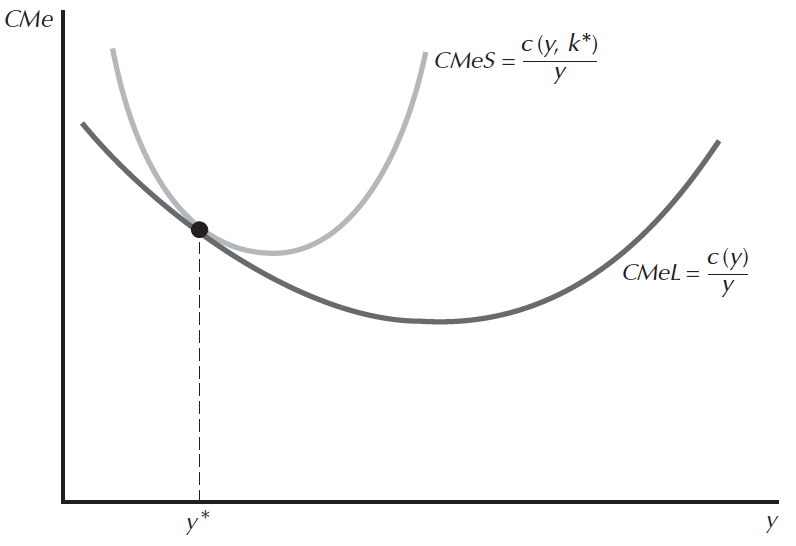
\includegraphics[width=3.8in]{figures4/shortlong1.png}
\end{center}
\end{frame}
\begin{frame}{Relaci\'on entre costos de corto y largo plazo}
\begin{itemize}
\item El proceso es el mismo cualquiera que sea el nivel de producción. Supongamos
que elegimos los niveles de producción $y_1, y_2, …, y_n$ y los tamaños de planta correspondientes $k_1 = k(y_1), k_2 = k(y_2),$ $ …, k_n = k(y_n)$. 
\item  El siguiente gr\'afico muestra que \textbf{la curva de costo medio a largo plazo es la envolvente de las curvas de costo medio a corto plazo}.
\end{itemize}
\end{frame}

\begin{frame}{Relaci\'on entre costos de corto y largo plazo}
	\begin{center}
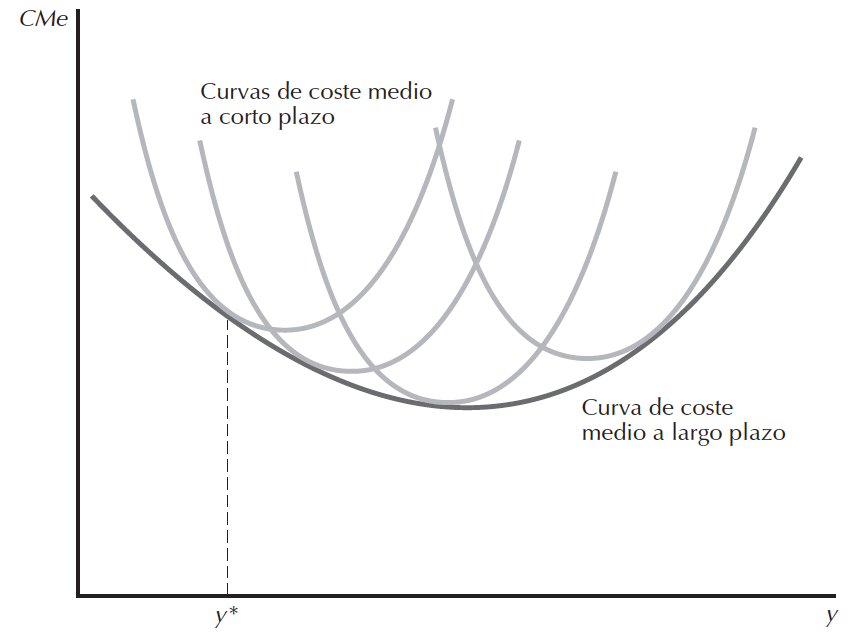
\includegraphics[width=3.8in]{figures4/shortlong2.png}
\end{center}
\end{frame}

\begin{solucion}


\begin{frame}{Relaci\'on entre costos de corto y largo plazo}
	\begin{center}
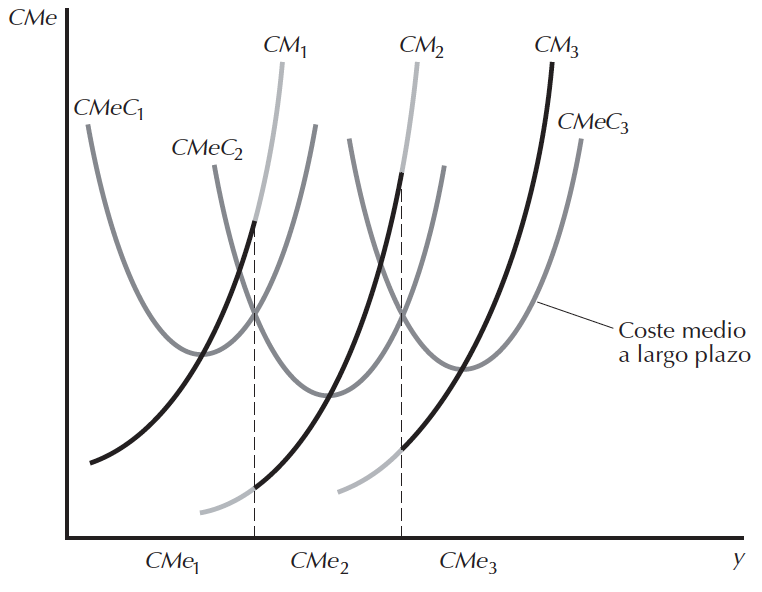
\includegraphics[width=3.8in]{figures4/shortlong3.png}
\end{center}
\end{frame}

\begin{frame}{Relaci\'on entre costos de corto y largo plazo}
	\begin{center}
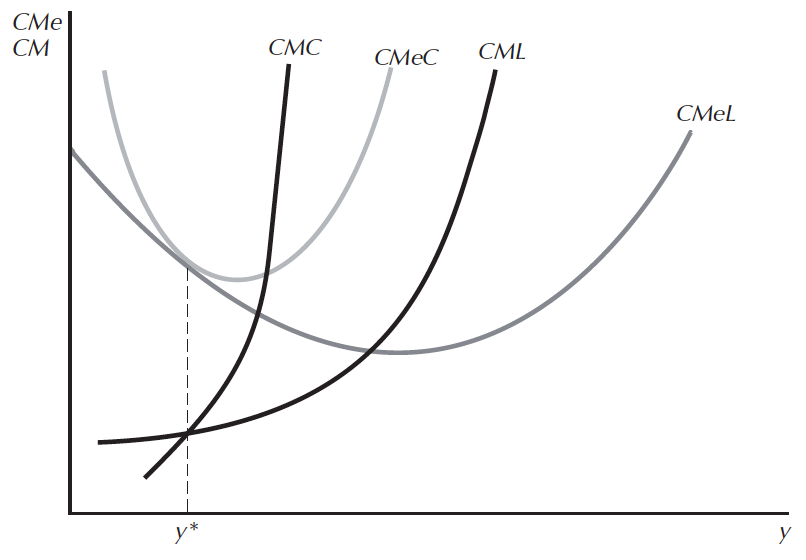
\includegraphics[width=3.8in]{figures4/shortlong4.png}
\end{center}
\end{frame}
\end{solucion}

\begin{frame}{¿Qué mide $\mu$?}
\begin{itemize}
%\item Relacionemos las soluciones de la maximización de beneficios y de la minimización de costos.
%\item  Las ecuaciones que caracterizan la soluci\'{o}n del problema de maximizaci\'{o}n de beneficios son:
%\begin{equation*}
%pPMg_{i}=w_{i}, \ \forall i
%\end{equation*}
\item Las condiciones que caracterizan la soluci\'{o}n del problema de minimizaci\'{o}n de costos:
\begin{align}
\mu ^{c}\left( w_{1},w_{2},y\right) PMg_{1}\left( w_{1},w_{2},y\right)
=&w_{1},\label{eq1} \\
\mu ^{c}\left( w_{1},w_{2},y\right) PMg_{2}\left( w_{1},w_{2},y\right)
=&w_{2}, \label{eq2}\\
f\left( x_{1}^{c}\left( w_{1},w_{2},y\right) ,x_{2}^{c}\left(
w_{1},w_{2},y\right) \right) =&y \label{eq3}
\end{align}
%\end{itemize}
%\end{frame}

%\begin{frame}{Relaci\'on entre min. de costos y max. de beneficios}
%\begin{itemize}
%\item Si bien no es inmediato que las soluciones a los problemas vayan a coincidir (pues a\'{u}n no determinamos la cantidad a producir en la segunda etapa luego de minimizar los costos), podemos comenzar por interpretar $\mu ^{c}$.
\item Consideremos la función de costos $C(w_1,w_2,y)$ y derivemos respecto a $y$
\begin{equation}
\frac{\partial C\left( w_{1},w_{2},y\right) }{\partial y}=\frac{\partial
x_{1}^{c}}{\partial y}\color{rosee}w_{1}\color{black}+\frac{\partial x_{2}^{c}}{\partial y}\color{rosee}w_{2}\color{black} \label{eq4}
\end{equation}
\item Reemplacemos (\ref{eq1}) y (\ref{eq2}) en (\ref{eq4}),
\begin{equation}
\frac{\partial C\left( w_{1},w_{2},y\right) }{\partial y}=\frac{\partial x_{1}^{c}}{\partial y}\color{rosee}\mu ^{c}PMg_{1}\color{black}+\frac{\partial x_{2}^{c}}{\partial y}\color{rosee}\mu ^{c}PMg_{2}\color{black} \label{eq5}
\end{equation}
\end{itemize}
\end{frame}

\begin{frame}{¿Qué mide $\mu$?}
\begin{itemize}
\item Derivando (\ref{eq3}) respecto de $y$ a ambos lados:
\begin{equation}
PMg_{1}\frac{\partial x_{1}^{c}}{\partial y}+PMg_{2}\frac{\partial x_{2}^{c}}{\partial y}=1 \label{eq6}
\end{equation}
\item Notemos que el lado derecho de (\ref{eq5}) es igual a $\mu^c$ multiplicado por el lado izquierdo de (\ref{eq6})
\begin{equation*}
\frac{\partial C\left( w_{1},w_{2},y\right) }{\partial y}=\underset{=1}{%
\underbrace{\left[ \frac{\partial x_{1}^{c}}{\partial y}PMg_{1}+\frac{%
\partial x_{2}^{c}}{\partial y}PMg_{2}\right] }}\mu ^{c}
\end{equation*}
\item Es decir,
\begin{equation*}
\frac{\partial C\left( w_{1},w_{2},y\right) }{\partial y}=CMg(y)=\mu^{c} 
\end{equation*}
\end{itemize}
\end{frame}

%\begin{frame}{¿Qué mide $\mu$?}
%\begin{itemize}
%\item Esto implica que en el \'{o}ptimo (cuando se eligen $x_1^c, x_2^c$ que minimizan costos) el valor del multiplicador de Lagrange, $\mu^c$ es igual al costo marginal. Es decir, es igual al aumento en el costo si la firma decidiera aumentar la producci\'{o}n. 
%\item Veremos a continuaci\'{o}n que debe ser cierto que el $CMg$ en el  \'{o}ptimo sea igual al precio del bien final. 

%\end{itemize}
%\end{frame}

\begin{frame}{Parte 2: Maximización de beneficios}
\begin{itemize}
\item \textbf{La soluci\'{o}n al problema de minimizaci\'{o}n de costos determina la mejor
manera de producir cualquier cantidad deseada de producto}.
\item \textbf{En la segunda etapa, el objetivo es elegir la cantidad a producir la que maximiza los
beneficios de la firma} (como tomadora de precios por el momento):
\begin{center}
$\max\limits_{y}py-C(y)$
\end{center}
\item Resolviendo este problema, la firma maximiza beneficios si:
\begin{align}
p=C'(y)=CMg(y) \label{eqmaxpi}
\end{align}
\item Para asegurarnos de que esta condici\'{o}n caracteriza un m\'{a}ximo debemos
verificar la \textbf{condici\'{o}n de segundo orden}, que aqu\'{\i} se resume a $C''(y)>0$, es decir, la funci\'{o}n de costos debe ser convexa (o el costo marginal creciente).
\end{itemize}
\end{frame}

\begin{frame}{Relaci\'on entre min. de costos y max. de beneficios}
\begin{itemize}
\item Para que se cumpla la CSO, la funci\'{o}n de costos tiene que ser estrictamente convexa, lo que implica que la funci\'{o}n de producci\'{o}n es estrictamente c\'{o}ncava en $y$. Recordemos que esta es la misma condición que pedíamos cuando vimos el problema de maximización de beneficios, pedíamos que $f(x_1,x_2)$ fuera estrictamente convexa en $(x_1,x_2)$.
\item Llamemos $y^{\ast}$ a la soluci\'{o}n del problema de maximizaci\'{o}n de
beneficios. Si en $y^{\ast}$ la tecnolog\'{\i}a tiene rendimientos no crecientes a escala, entonces:
\begin{center}
$CMg(y^{\ast })\geq CMe(y^{\ast })$
\end{center}
\item Lo que implica que los beneficios de la firma son no negativos:
\begin{center}
$py^{\ast }-C(y^{\ast })=y^{\ast}(CMg(y^{\ast })-CMe(y^{\ast }))\geq 0$
\end{center}
\end{itemize}
\end{frame}

\begin{frame}{Maximización de beneficios con tecnología CRS}
\begin{itemize}
\item \textquestiondown Qu\'{e} pasa cuando la tecnolog\'{\i}a tiene rendimientos
constantes a escala? 
\item En ese caso, $C(y)=cy$ y el beneficio de la firma es:
\begin{center}
$\pi =(p-c)y$
\end{center}
\item Por lo tanto, si $p>c$ el problema no tiene soluci\'{o}n $(y\rightarrow
\infty)$.
\item Si $p=c$, el problema tiene infinitas soluciones $(y\in \mathbb{R}^{+})$.
\item Si $p<c$, el problema tiene una \'{u}nica soluci\'{o}n, $y=0$.
\end{itemize}
\end{frame}


\begin{solucion}
\begin{frame}{Demanda que enfrenta una firma}
\begin{itemize}
\item Notemos que en un mercado perfectamente competitivo, dado que hay muchas firmas compitiendo en el mercado, hay una diferencia entre la \textbf{demanda que enfrenta una firma} y la \textbf{demanda de mercado}. La primera mide la relación entre el precio de mercado y la producción de una firma específica. La segunda mide la relación entre el precio de mercado y la cantidad total vendida.
\item La curva de demanda del mercado depende de la conducta de los consumidores. La
curva de demanda a la que se enfrenta una firma no depende sólo de la conducta de
los consumidores, sino también de la conducta de las demás firmas. 
\item En un mercado competitivo cuando hay muchas firmas pequeñas, que son tomadoras de precios,
cada una se enfrenta a una curva de demanda horizontal.
\end{itemize}
\end{frame}

\begin{frame}{Demanda que enfrenta una firma}
	\begin{center}
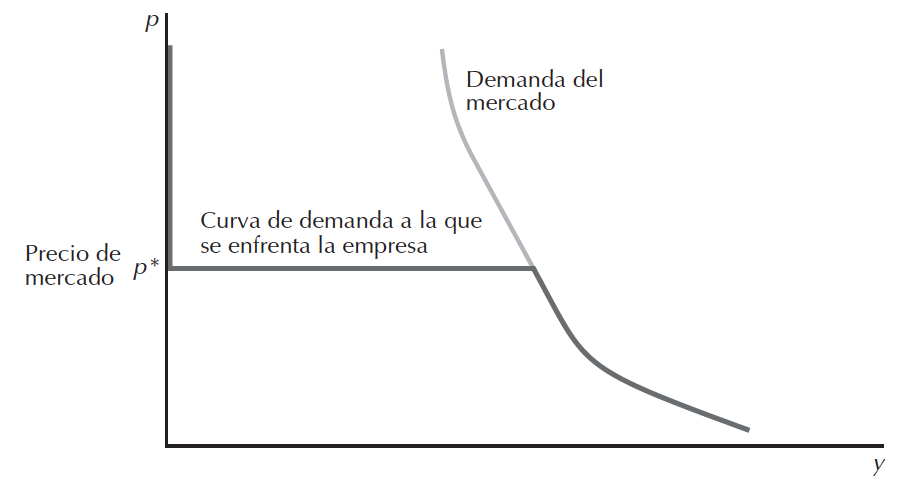
\includegraphics[width=4in]{figures4/demanda.png}
\end{center}
\end{frame}
\end{solucion}

\begin{frame}{Oferta: corto plazo}
\begin{itemize}
\item Volviendo al caso general, para conocer la función de oferta de la firma, nos preguntamos: \textbf{¿Qué condición de optimalidad determina la cantidad que la firma decidirá producir?}

\item La firma produce una cantidad $y$ de manera que $IMg(y)=CMg(y)$. \textit{Si no se cumple esta condición, la firma siempre podrá aumentar sus beneficios modificando cuánto produce (excepto si produce $y=0$).} %, en la que el ingreso adicional generado por una unidad más de producción sea exactamente igual al costo adicional de esa unidad.

\item En competencia perfecta, $IMg(y)=p$. Por eso, $p=CMg(y)$, como vimos en (\ref{eqmaxpi}).

\item $p=CMg(y)$ nos dice cuántas unidades $y$ ofrece la firma cuando el precio es $p$. Por lo tanto, \textbf{la curva de costo marginal de una firma competitiva es su curva de oferta}. Una firma perfectamente competitiva vende $y$ unidades a precio $p$ cuando $p$ es igual al costo marginal de producir la última unidad $CMg(y)$. 
\item Nos quedan por responder: ¿puede haber bienes Giffen? ¿A partir de qué precio mínimo ofrece la firma $y>0$? %En otras palabras, el precio de mercado es precisamente el costo marginal, siempre y cuando cada firma esté produciendo en su nivel maximizador del beneficio.
\end{itemize}
\end{frame}

\begin{frame}{Oferta: ¿Puede haber bienes Giffen?}
\begin{itemize}
\item Consideremos el siguiente caso:
\begin{center}
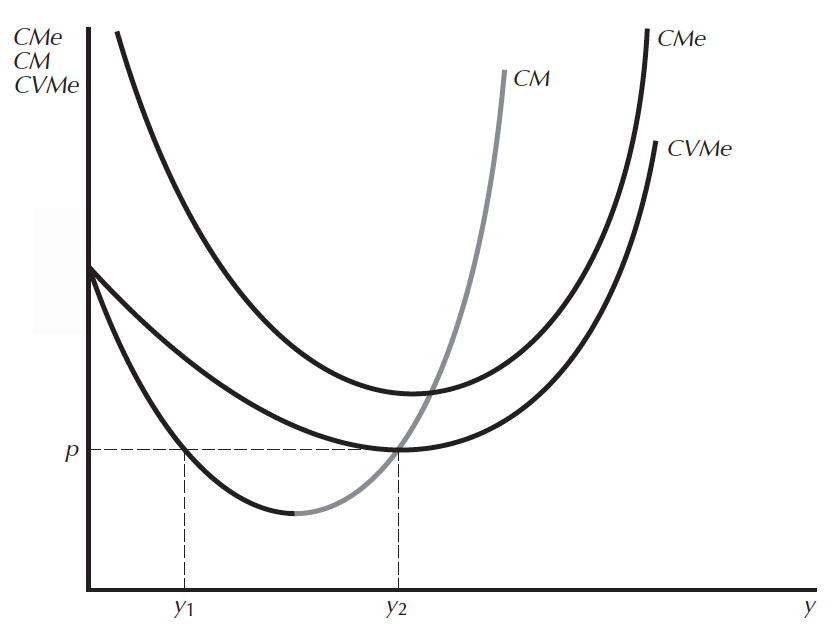
\includegraphics[width=3.5in]{figures4/doble.png}
\end{center}
\end{itemize}
\end{frame}

\begin{frame}{Oferta: ¿Puede haber bienes Giffen? NO}
\begin{itemize}
\item Para el precio $p$, en la curva $CMg$ hay dos cantidades, $y_1$ e $y_2$ que cumplen que $CMg(y)=p$. Si la firma considerase producir $y_1$, la curva de costo marginal es decreciente. Si aumentásemos la producción, disminuirán los costos marginales. Podríamos tener beneficios mayores produciendo $y_2$. %\textbf{ ... no me gusta como estaba escrito pero tampoco como lo estoy escribiendo}

%Pero el precio de mercado continuará siendo el mismo y, por lo tanto, es evidente que aumentarán los beneficios.
%\item Por consiguiente, podemos excluir los niveles de producción en los que la curva de costo marginal tiene pendiente negativa. En esos puntos, el incremento de la producción aumentará los beneficios. 
\item \textbf{La curva de oferta de una firma competitiva va a estar dentro de la parte creciente de la curva de costo marginal}. La curva de oferta oferta tiene pendiente positiva. \textbf{Por lo tanto, no puede haber bienes Giffen en las curvas de oferta.}
\item Nos queda ver para qué valores de $y$ (donde $CMg(y)$ es creciente) la firma estará dispuesta a ofrecer $y>0$. 
\end{itemize}
\end{frame}

\begin{frame}{Oferta: ¿a partir de qué precios se ofrece $y>0$?}
\begin{itemize}
\item Si bien $p=CMg(y)$ \textbf{es una condición necesaria} para maximizar beneficios, no siempre es suficiente. %El mero hecho de que hallemos un punto en el que el precio sea igual al costo marginal no significa que hayamos encontrado el punto de máximo beneficio. Sin embargo, si encontramos el punto de máximo beneficio, sabemos que el precio debe ser igual al costo marginal.
\item Como la firma tiene siempre la opción de no producir, tenemos que comparar que que los beneficios de producir sean efectivamente mayores a los de no producir.
\item \textbf{En el corto plazo, si una firma produce una cantidad nula, tiene que seguir pagando los costos fijos}
$F$. Por lo tanto, los beneficios que genera la producción de cero unidades son $– F$. Los beneficios que genera la producción de una cantidad $y$ son $py – c_v(y) – F$. 
\item La firma mejora su situación cerrando cuando:
\begin{center}
$-F>py – c_v(y) – F \Leftrightarrow CMeV(y)=\dfrac{c_v(y)}{y}>p$
\end{center}
\item Esta se conoce como \textit{la condici\'on de cierre}.
\end{itemize}
\end{frame}
\begin{frame}{Oferta: corto plazo}
\begin{itemize}
\item Por lo tanto, la firma sólo ofrecerá cantidades $y>0$ siempre y cuando $CMg(y)>CMeV(y)$. 

\item Gráficamente, la firma ofrecerá cantidades $y$ solamente a partir de que la curva $CMg$ esté arriba de la curva $CMeV$. 

\item Si el precio $p$ al que la firma pudiese vender el bien final $y$ cumpliese que $p=CMg(y)<CMeV(y)$, la decisión óptima de la firma consistiría en producir cero unidades.

\item Por lo tanto, la firma ofrecerá cantidades $y$ que cumplan que $p=CMg(y)$ si $p>CMe_{min}$.
\end{itemize}
\end{frame}

\begin{frame}{Oferta: corto plazo}
\begin{center}
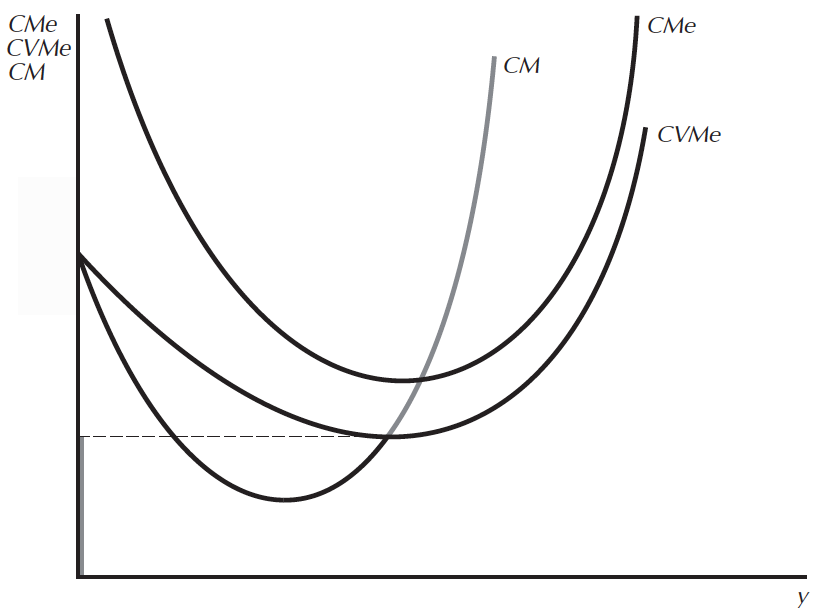
\includegraphics[width=3.8in]{figures4/oferta.png}
\end{center}
\end{frame}

\begin{frame}{Beneficios}
\begin{itemize}
\item Para ver gráficamente los beneficios $\pi=IT-CT$:

\begin{enumerate}
    \item obtenemos una expresión para los ingresos totales $IT$: $IT=p\cdot y=CMg(y)\cdot y$. Los $IT$ se miden con el \'area del rectángulo que tiene base $y$ y altura $CMg(y)$.
    \item obtenemos una expresión para los costos totales $CT$: $CT=CMe(y)\cdot y=$. Los $CT$ se miden con el \'area del rectángulo que tiene base $y$ y altura $CMe(y)$.
\end{enumerate} 
\item Los beneficios, son simplemente la diferencia entre ambos, 

\[\pi =(CMg(y)-CMe(y))\cdot y.\]
\end{itemize}
\end{frame}

\begin{frame}{Beneficios y excedente del productor}
\begin{center}
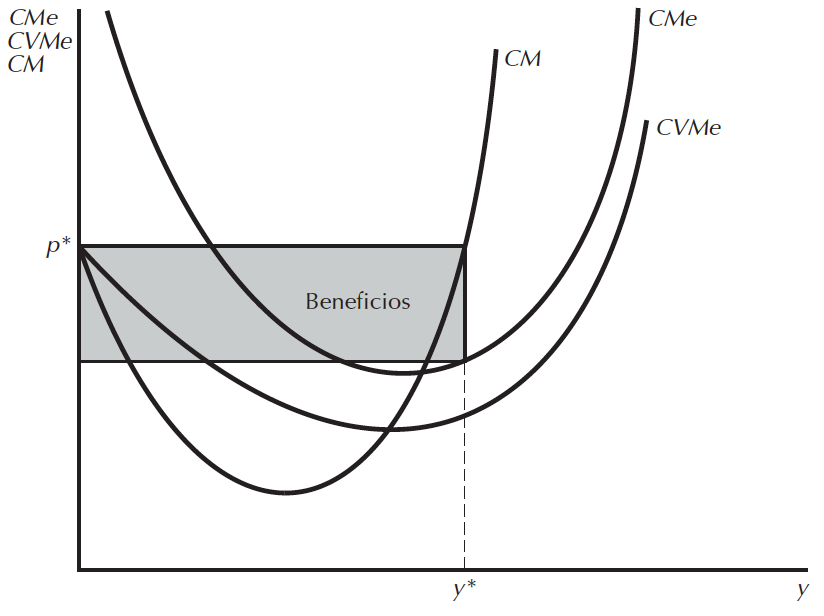
\includegraphics[width=3.8in]{figures4/beneficios.png}
\end{center}
\end{frame}

\begin{frame}{Beneficios: corto plazo}
    \begin{itemize}
        \item Notemos que en el corto plazo puede haber firmas con beneficios negativos, positivos o nulos.
    \end{itemize}
\begin{center}
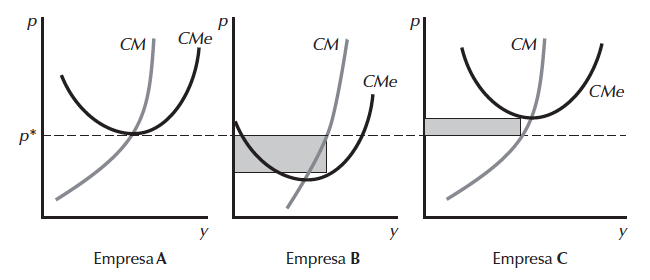
\includegraphics[width=3.8in]{figures5/industry_profits.png}
\end{center}
\end{frame}

\begin{frame}{Beneficios y excedente del productor}
\begin{itemize}
\item En el corto
plazo, una firma no necesariamente obtiene beneficios positivos. Por ejemplo, en el caso B, el precio $p$ es lo suficientemente grande para que $p>\frac{c_{v}\left(
y\right) }{y}$ (para que la firma decida producir) pero menor al m\'{i}nimo costo medio total. El objetivo de dicha producci\'{o}n es ``minimizar las p\'{e}rdidas''. Se busca perder menos que $F$.
\item El \textbf{excedente del productor} (EP) es otra medida de bienestar de la firma. Es el ingreso extra que la firma obtiene por operar en una econom\'{i}a de mercado en donde todas sus unidades se venden al mismo precio.

\begin{enumerate}[label=\textbf{(\Alph*)}]
    \item $EP=IT-CV$, ingresos menos
los costos variables.
    \item $EP=\pi+F$, beneficios más los costos fijos
    \item $EP=\displaystyle\int\limits_{p_{0}}^{p}y\left( p\right) dp$ donde $p_{0}=CMeV_{min}$. Noten que la integral definida sobre el eje vertical.
\end{enumerate}
\end{itemize}
\end{frame}
\begin{solucion}
\begin{frame}{Beneficios y excedente del productor}
\begin{itemize}
\item La manera más directa de medir el excedente del productor consiste en hallar la
diferencia entre el rectángulo de los ingresos y el rectángulo $y^*CVMe(y^*)$ de la figura
anterior. 
\item Pero hay una forma más útil de medirlo: mediante la propia curva de costo
marginal. Vimos que el área situada debajo de la curva de costo marginal medía los costos variables totales, debido a que representa el costo que genera producir la primera unidad más el costo que genera producir la segunda, etc. Así, para hallar el excedente del productor, podemos restar esa área de la del rectángulo de ingreso.
\end{itemize}
\end{frame}
\end{solucion}

%\begin{frame}{Beneficios y excedente del productor}
%\begin{itemize}
%\item Por último, podemos combinar las dos maneras de medir el excedente del productor. Utilicemos la definición basada en el rectángulo hasta el punto en el que el costo marginal es igual al costo variable medio y a continuación el área situada encima de la curva de costo marginal. Este método es el más útil en la mayoría de los casos, ya que es precisamente el área situada a la izquierda de la curva de oferta:
%\begin{equation*}
%EP=\int\limits_{p_{0}}^{p}y\left( p\right) dp
%\end{equation*}
%donde $p_{0}$ es el precio tal que la firma comienza a ofrecer en el corto plazo. Noten que la integral definida sobre el eje vertical.
%\end{itemize}
%\end{frame}

\begin{frame}{Beneficios y excedente del productor}
\begin{center}
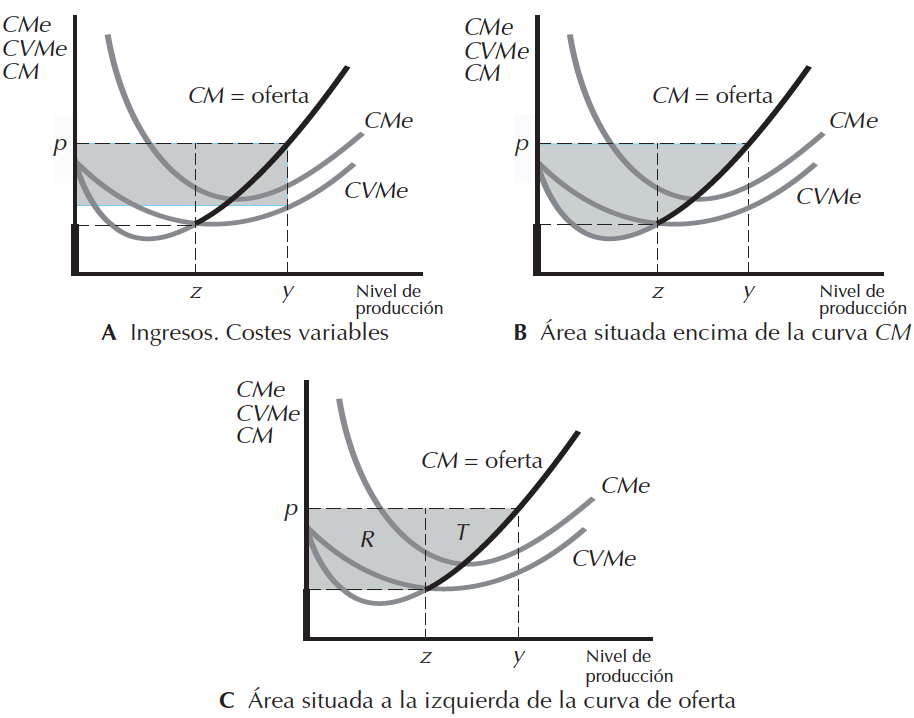
\includegraphics[width=3.8in]{figures4/EP.png}
\end{center}
\end{frame}


\begin{frame}{Variaci\'on en el excedente del productor}
Si el precio pasa de $p^*$ a $p^{'}$, el $EP$ varía y esa medición nos da una idea del cambio en el bienestar del productor.
\begin{center}
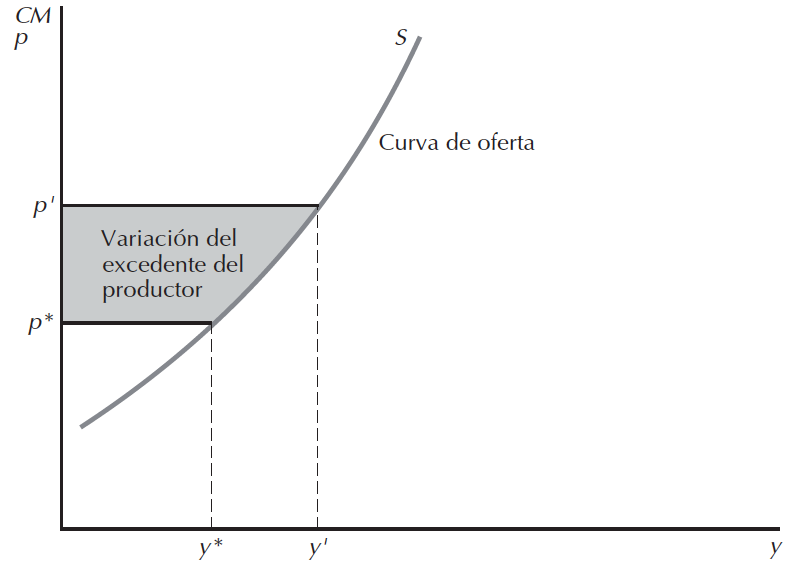
\includegraphics[width=3.5in]{figures4/varEP.png}
\end{center}
\end{frame}

\begin{frame}{Variaci\'on en el excedente del productor}
\begin{itemize}
\item Notemos que la variación en el excedente del productor cuando la firma pasa de producir de $y^*$ a $y'$ es exactamente igual que la variación que experimentan los beneficios en la misma situación, ya que, por definición, los costos fijos
no varían. 
\item Por lo tanto, basándonos en la información que proporciona la curva de
costo marginal, podemos medir el efecto que produce en los beneficios una variación de la producción.
\end{itemize}
\end{frame}

\begin{frame}{Oferta: largo plazo}
\begin{itemize}
\item La función de \textbf{oferta de largo plazo} de la firma nos da la relación entre cada precio $p$ y la cantidad la cantidad $y$ que produce óptimamente (maximizando beneficios de LP) cuando la firma puede elegir incluso los factores que son fijos a corto plazo. Es decir, la curva de oferta de largo plazo es:
\begin{center}
$p = CMg_L(y) = CMg(y, k(y))$
\end{center}
\item Para obtener la curva de oferta a corto plazo hay que considerar la igualdad del precio
y el costo marginal dado algún valor para $k$—no necesariamente $k(y)$:
\begin{center}
$p = CMg(y, k)$
\end{center}
\item Notemos la diferencia entre las dos expresiones. La curva de oferta a corto plazo
depende del costo marginal de producción dado algún valor de $k$, mientras que la curva de
oferta a largo plazo depende del costo marginal de producción correspondiente al nivel
óptimo $k=k(y)$.
\end{itemize}
\end{frame}

\begin{frame}{Oferta: largo plazo (LP)}
\begin{itemize}
\item Consideremos $y^*$, la cantidad producida para maximizar beneficios de LP para un precio $p^*$ y $k^*$, la cantidad de insumo $2$ que se utiliza para maximizar beneficios de LP.
\item %Sabemos algo sobre la relación entre los costos marginales a corto plazo y a largo plazo: 
Los costos marginales a corto y a largo plazo coinciden en el nivel de producción $y^*$, si el factor fijo en el corto plazo es igual a $k^*$.
\item Por lo tanto, para la cantidad $y^*$ las curvas de oferta de corto plazo y de largo plazo se intersecan en $(y^*,p^*)$ sin el factor fijo de corto plazo es $k=k^*$.
\item %En el corto plazo, la firma tiene algunos factores cuya oferta es fija; a largo plazo, todos son variables. 
Para otros valores de $p\neq p^*$, en el largo plazo la firma tiene más posibilidades de elegir insumos óptimamente que a corto plazo, lo que iimplica que \textbf{la curva de oferta a largo plazo es más sensible al precio (más elástica) que la curva de oferta a corto plazo}. Esto ocurre porque la cantidad ofrecida puede potencialmente cambiar más ante un cambio en el precio.
\end{itemize}
\end{frame}

\begin{frame}{Oferta: largo plazo}
\begin{center}
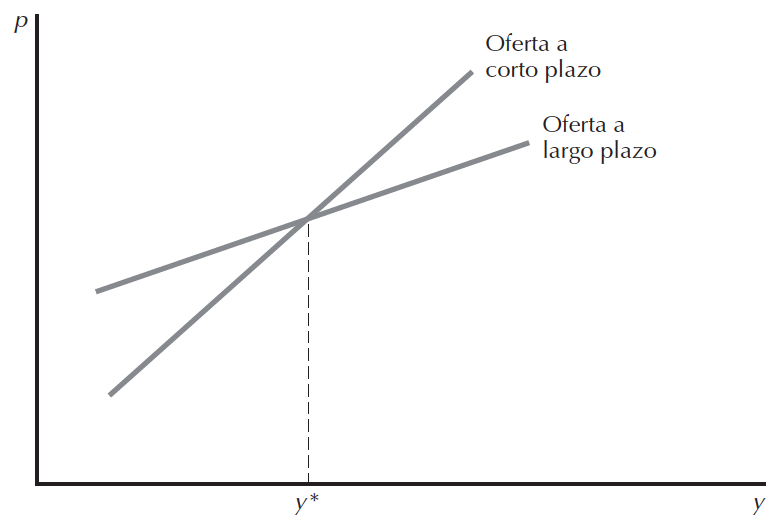
\includegraphics[width=3.8in]{figures4/LP.png}
\end{center}
\end{frame}

\begin{frame}{Oferta: largo plazo. ¿salir o quedarse en el mercado?}
\begin{itemize}
%\item ¿Qué más podemos decir sobre la curva de oferta a largo plazo? 
\item  La firma tiene dos opciones en el mercado: \textbf{continuar produciendo o salir del mercado}. Dado que a largo plazo siempre puede obtener
cero beneficios abandonando el mercado, si la firma decidiera producir los \textbf{beneficios que obtiene en el
largo plazo tienen que ser al menos cero}:
\begin{center}
$py-C(y)\geq 0 \Leftrightarrow p\geq CMe(y)$
\end{center}
\item Por lo tanto, la firma empezará a ofrecer cantidades positivas solamente si $p\geq CMe_{min}$. %la parte relevante de la curva de oferta a largo plazo es la parte creciente de la curva de costo marginal que se encuentra por encima de la curva de costo medio a largo plazo.
\end{itemize}
\end{frame}

\begin{frame}{Oferta: largo plazo}
\begin{center}
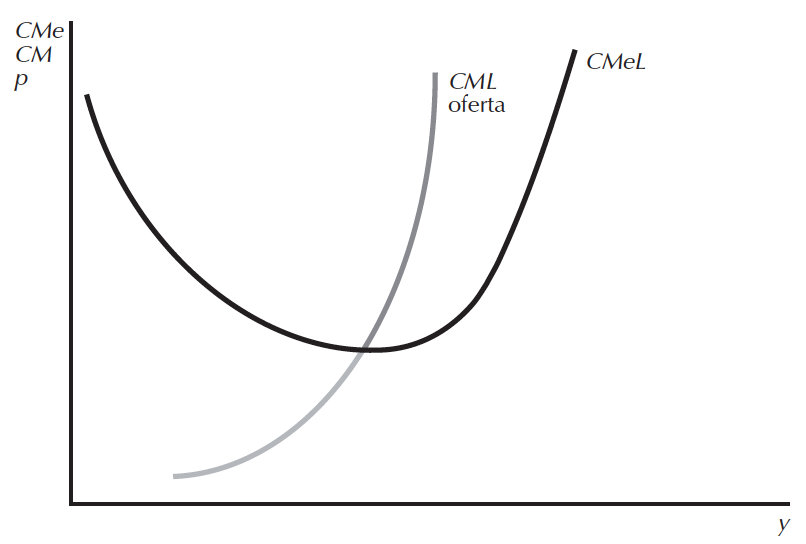
\includegraphics[width=3.8in]{figures4/cmgLP.png}
\end{center}
\end{frame}

\begin{frame}{Funci\'on de oferta en el largo plazo con CRS}
\begin{itemize}
\item Si la tecnología a largo plazo de la firma tiene rendimientos constantes de escala, la curva de oferta a largo es una recta horizontal. ¿Por qué?

\item Como $C(y)=cy$, entonces $CMe(y)=CMg(y)=c$, por lo tanto la curva de costo marginal es igual a la curva de costo medio en el largo plazo. %Esto ocurre porque, cuando los costos medios son constantes, la curva de costo marginal coincide con la curva de costo medio a largo plazo.

\item Por lo tanto, la que la curva de oferta a
largo plazo es una recta horizontal en $c$.
\item La firma está dispuesta a ofrecer cualquier
cantidad de producción si $p = c$, una cantidad arbitrariamente grande si $p > c$ y una cantidad nula si $p < c$.
\end{itemize}
\end{frame}

\begin{frame}{Funci\'on de oferta en el largo plazo con CRS}
\begin{center}
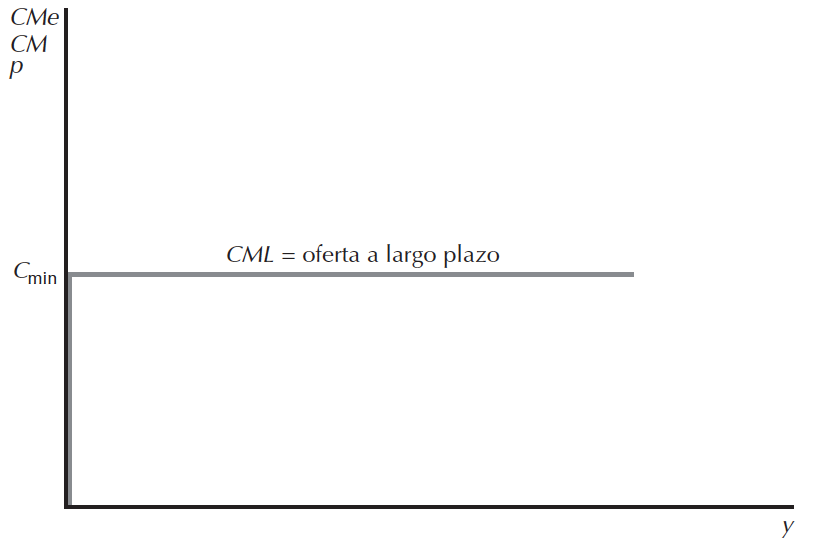
\includegraphics[width=3.8in]{figures4/RCSLP.png}
\end{center}
\end{frame}


\begin{frame}{Oferta de la industria: largo plazo}
    \begin{itemize}
        \item En el largo plazo, las firmas pueden elegir las cantidades de todos sus insumos.
        \item Hay otro efecto a considerar en el largo plazo: la entrada y salida de firmas del mercado. Si permitimos que eso ocurra, decimos que hay \textbf{libre entrada y salida} de firmas.
        \item Si una firma pierde dinero en el largo plazo, puede salir del mercado. De la misma manera, si las firmas se encuentran obteniendo beneficios positivos en el largo plazo, esperaremos que más firmas ingresen al mercado, dado que todas las firmas tienen acceso a la tecnología de producción.
    \end{itemize}
\end{frame}

\begin{frame}{Oferta de la industria: largo plazo - Firmas idénticas}
\begin{itemize}
\item Supongamos que todas las firmas cuentan con la misma tecnología de producción, y por lo tanto idéntica función de costos $C(y)$.
\item Llamemos $y^{*}$ al nivel de producto que minimiza los costos medios de largo plazo y $CMe_{min} = \dfrac{C(y^{*})}{y^{*}}$ al costo medio mínimo.
\item Notemos que si $p > CME_{min}$, entonces nuevas firmas desearán entrar al mercado, ya que habrá beneficios positivos.
\item La entrada de nuevas firmas hace que la curva de oferta de la industria se vuelva más horizontal y hace que el precio de equilibrio de mercado de largo plazo sea menor. 
\item Por lo tanto, en el largo plazo el precio vendrá dado por $p^{*}= CMe_{min}$ y cada firma producirá $y^{*}$. La cantidad de firmas en el mercado será la variable endógena a determinar.
\end{itemize}
\end{frame}

\begin{frame}{Oferta de la industria: corto plazo}
 Una vez que encontramos la oferta de la firma podemos encontrar la oferta de la industria sumando las ofertas individuales de las $n$ firmas (suponiendo que el número de firmas se mantiene fijo): $S(p) = \sum_{i=1}^{n}s_{i}(p)$
    
    


    \begin{center}
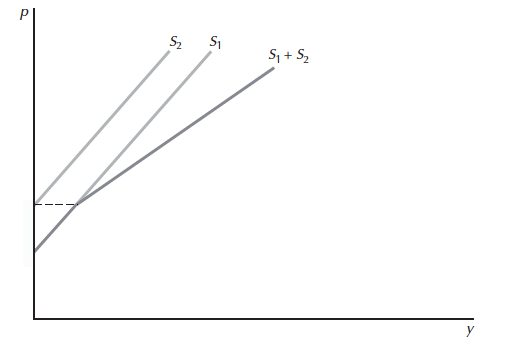
\includegraphics[scale=0.5]{figures5/industry_offer.png}
\end{center}
\end{frame}

\begin{frame}{Equilibrio de largo plazo}
\begin{itemize}
 \item   Cuando hay libre entrada y salida de firmas, porque las firmas pueden decidir entrar o salir, un equilibrio se compondrá de tres cosas:
    \begin{enumerate}
    \item precio $p^*$ de equilibrio
    \item cantidad $y^*$ de equilibrio
    \item cantidad $n^*$ de firmas que venden en equilibrio.
    \end{enumerate}
    
    \item Suponiendo que todas las firmas son iguales, $S(p) = \sum_{i=1}^{n}s_{i}(p)=ns_1(p)$
    
    la idea sería encontrar $(p,^*,y^*,n^*)$ que cumplan que: 
    
\begin{align*}
    ns_1(p)=D(p)\\
    \pi(p)=0
\end{align*}

\item La primera condición dice que oferta de mercado es igual a demanda de mercado. La segunda condición dice que entran firmas hasta que los beneficios sean cero. Esto es porque si fueran positivos más firmas querrían empezar a producir y si los beneficios fueran negativos habría firmas que querrían dejar de producir.
    
    \end{itemize}
\end{frame}
\end{document}